\documentclass{article}
\usepackage{tikz}
\usetikzlibrary{arrows}
\usepackage{pgfplots}
\usepackage{amsmath}
\usetikzlibrary{datavisualization}
\usetikzlibrary{datavisualization.formats.functions}
\usepackage{cite}
\begin{document}
	\title{Test Problem3}
	\author{Rashi}
	\date{\today}
	\maketitle
	\section{Plotting graphs from equation}
	Following is an example of plotting graph from the equation.\\
	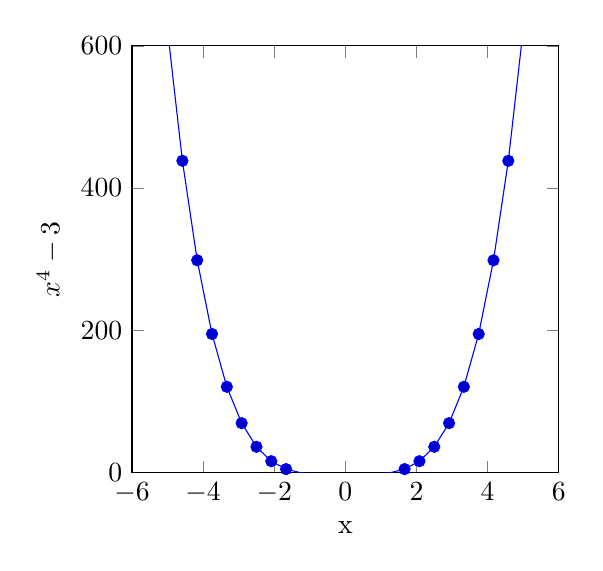
\begin{tikzpicture}
	\begin{axis}[ymin=0,xmin=-6,ymax=600,xmax=6,ytick distance=200,xtick distance=2,height=7cm,width=7cm,xlabel=x,ylabel=$x^4-3$]
	\addplot expression{x^4-3};		
	\end{axis}
	\end{tikzpicture}\\
	Following are the examples of plotting more than one equations in a sigle dia-
	gram. To plot from the equaions use the package ”pgfplots” Specify the domain
	as shown in the diagram.

	
	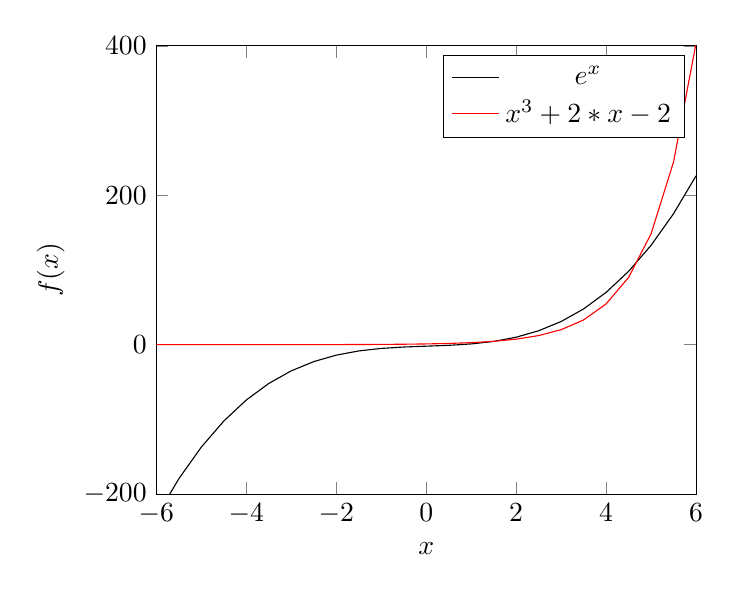
\begin{tikzpicture}
	\begin{axis}[xlabel=$x$,ylabel=$f(x)$,ymin=-200,ymax=400,xmin=-6,xmax=6,ytick distance=200,xtick distance=2,legend entries={$e^{x}$, $x^3 + 2*x -2$}]
	\addplot[mark=none,domain=-6:6]{x^3 + 2*x -2} ;
	\addplot+[mark=none,domain=-6:6]  {exp(x)};
	\end{axis}
	\end{tikzpicture}
	\section{Bibliography in LaTex}
	
	Bibliography is created by using BibTex \cite{1}. BibTeX is reference management
	software for formatting lists of references \cite{2} The BibTeX is a stand-alone utility
	or tool typically used together with the LaTeX document preparation system.
	It was developed by Oren Patashnik \cite{3}.
	\bibliography{Problem3}
	\bibliographystyle{unsrt}
\end{document}